% Copyright 2021 Jacopo Maltagliati
%
% Use of this source code is governed by an EUPL-style
% license that can be found in the LICENSE file or at
% https://eupl.eu/1.2/en/.
% A localized copy of this license can be found in the LICENSE.it file or at
% https://eupl.eu/1.2/it/
%
% Portions of this document are subject to different licensing agreements,
% see src/titlepage.tex for details.

\documentclass[a4paper,12pt]{report}
\usepackage[paper=a4paper,margin=1in]{geometry}
\usepackage{graphicx}
\usepackage{float}
%\usepackage{hyperref}
\usepackage[T1]{fontenc}
\usepackage{lmodern}
\usepackage[utf8]{inputenc}
\usepackage{setspace}
\usepackage[english]{babel}
%\usepackage{amssymb}
%\usepackage{amsthm}
%\usepackage{amsmath}
%\usepackage{amstext}
\usepackage{microtype}
\usepackage{csquotes}
\usepackage{bookmark}
\usepackage{xpatch}
\usepackage{listings}
\usepackage{minted}
\usemintedstyle{borland}
\usepackage[backend=biber, sorting=none]{biblatex}
\hypersetup{colorlinks=true, linkcolor=blue, citecolor=blue, urlcolor=blue, pdftitle={Linux as a Real-Time Operating System}}
\addbibresource{all.bib}
\usepackage[color=green,textsize=tiny]{todonotes}
\usepackage{sectsty}
\chapternumberfont{\large}
\chaptertitlefont{\huge}
\renewcommand{\familydefault}{\sfdefault}
\newcommand{\comment}[1]{}
\begin{document}
% Titlepage
% Copyright 2020 Luca Chiodini
%
% Use of this source code is governed by an MIT-style
% license that can be found in the LICENSE file or at
% https://opensource.org/licenses/MIT.
%
% The Università degli Studi di Milano-Bicocca "ottaedro leonardesco" logo is
% protected by copyright, and it can be used under the terms and conditions
% that can be found in the logo-license.pdf file, or at
% https://www.unimib.it/sites/default/files/Allegati/regolamento.pdf.

\begin{titlepage}

    \noindent
    \begin{minipage}[t]{0.19\textwidth}
        \vspace{-4mm}{\includegraphics[scale=1.15]{logo.pdf}}
    \end{minipage}
    \begin{minipage}[t]{0.81\textwidth}
        {
            \setstretch{1.42}
            {\textsc{Università degli Studi di Milano - Bicocca}} \\
            \textbf{Scuola di Scienze} \\
            \textbf{Dipartimento di Informatica, Sistemistica e Comunicazione} \\
            \textbf{Corso di laurea in Informatica} \\
            \par
        }
    \end{minipage}

    \vspace{35mm}

    \begin{center}
        {\Huge{
                \setstretch{1.2}
                \textbf{Linux as a Real-Time Operating System: a practical analysis in the mobile robotics domain}
                \par
            }
        }
    \end{center}

    \vspace{30mm}

    \noindent
    {\large \textbf{Relatore:} Prof. Sorrenti Domenico } \\

    \noindent
    {\large \textbf{Co-relatore:} Prof. Braione Pietro } \\
    
    \noindent
    {\large \textbf{Co-relatore:} Prof. Ferretti Claudio }

    \vspace{15mm}

    \begin{flushright}
        {\large \textbf{Relazione della prova finale di:}} \\
        \large{Jacopo Maltagliati} \\
        \large{Matricola 830110}
    \end{flushright}

    \vspace{2mm}

    \begin{center}
        {\large{\bf Anno Accademico 2019-2020}}
    \end{center}

    \restoregeometry

\end{titlepage}
\newpage
% Quote
\vspace*{\stretch{1}}
\begin{flushright}
  \itshape
  \begin{tabular}{@{}l@{}}
    In (conflicted) memory of Fulvio Testi 174.\\
    2017-2020\\ JM,MP,MS,MT,AM,MC 
  \end{tabular}
\end{flushright}
\vspace{\stretch{2}}
\newpage
% Toc
\tableofcontents
\newpage
% Set paragraph spacing so our eyes don't pop while reading
\setlength{\parskip}{1em}
% Ch0
\chapter*{Acknowledgements}
A special thanks for the continued support and previous work on Otto, ROS and the USAD platform goes to Domenico Sorrenti, Federica Di Lauro, Simone Fontana, Carlo Radice, Giovanni Capra and Riccardo Curnis of the IRAlab team, and to the former IRAlab member Augusto Luis Ballardini.

% Ch1
\chapter{Summary}

In the past ten years, mobile robotics as a field has been gaining a lot of traction: as technology evolves, building a mobile platform has become more and more feasible for anyone, including small research teams and hobbyists. However, there is still a lack of easily approachable real-time solutions able to manage the workload, as many of the available frameworks are not mature enough to offer fine-grained real time application control: this is why we ultimately decided to push the Linux kernel to its limits, studying its real-time capabilities and ease of use.

\section{The problem}

Imagine driving on an empty road at night while listening to classical music: it's been a very long day, and your consciousness gradually drifts to a peaceful slumber. Suddenly, an animal crosses the road: are you going to notice? Will you be able to stop in time? Now, consider a self-driving car in the same situation: what would happen if the control computer "dozed off" even for a fraction of a second? The user would probably not be able to stomp on the brakes fast enough to prevent the car from crashing.

A possible solution to this problem is carefully designing a system built around existing technologies, such as real-time control, redundant hardware platforms, and failsafe mechanisms. However, creating a real-time system from the ground up tends to be very expensive and error-prone, as incorrect design or minor mistakes could lead to catastrophic failures such as the infamous Therac \cite{therac-25-accidents} incidents.

For this reason, many software houses have been working on various commercial solutions since the 1980s that enabled programmers and engineers to deploy their application on proven grounds, thus reducing the time and effort needed to create a real-time application. Arguably, the best aspect of those systems was their widespread availability: for example, DEC's VAXeln used lightly modified VAX computers, and Quantum Computer Inc. QNX ran on consumer-grade hardware, including x86 processors. While the VAXeln is now a historical platform, QNX is still commercially available from BlackBerry Limited and major companies such as Apple use it for their products \cite{time-carplay-qnx}.

However, having always demonstrated an incredible flexibility, the ubiquitous Linux kernel is becoming a viable option for robotics and real-time usage, with both academic and commercial applications exploiting it like Tesla Motors, which maintains its own fork \cite{gh-tesla-linux}.

Of course, this flexibility comes at the cost of reduced effectiveness in each specific situation, so why do both academic and commercial researchers decide to use Linux? For example:
\begin{itemize}
  \item Linux is free and comes at no cost.
  \item Linux is open-source, so it might be tailored to specific needs with the right expertise.
  \item Linux has a wide community of people constantly improving it, ensuring constant updates without any support contract.
\end{itemize}

These, along with the fact that IRAlab has been running Linux on control systems for several years, are the reasons why we decided to adopt it for this project.

\section{The current implementation}

At the moment, most of IRAlab's mobile platforms are controlled by a master node running Ubuntu Linux 16.04 LTS and the ROS framework, which was created by Willow Garage as a rapid development platform for their PR2 robot and traces its roots into an even earlier effort by a team of researchers and students at Stanford University. 

The name "Robot Operating System" is misleading: in fact, ROS is mostly an open-source middleware, that is a set of software libraries and tools that help you build robot applications, which actually needs an underlying operating system to run: currently, it may do so on both Unix-like operating systems such as Ubuntu GNU/Linux, BlackBerry QNX \cite{qnx-ros} and Apple macOS, and on some Microsoft Windows versions. For simplicity, throughout this report we'll use the term "ROS" to refer to the ROS+Linux combination.

\subsection{Description}

Currently, IRAlab mainly uses a modified ROS navigation stack for abstraction and rapid prototyping: through the use of \textit{topics} and \textit{messages}, ROS provides a facility to let the users write small programs, called \textit{nodes}, and make them communicate with each other. A \textit{master node}, provided by the framework, acts as a central hub, keeping tabs on the state of the \textit{Computational Graph}. Moreover, ROS provides extensive \textit{timestamping} and data logging facilities, letting the user easily track, monitor and simulate a mobile platform's behavior.

An in-depth analysis of the ROS functionalities and usage in the context of our mobile platforms is beyond the scope of this report, but the same topic has received extensive coverage in earlier works by Gerosa* and Di Lauro \cite{fdila-bs-otto}.
\todo{dilauro -> ???}

\subsection{Issues}

The problem we encountered with ROS is its complexity: while it's a easily modifiable and extensible, there is no simple way to control precisely how the nodes are scheduled. Finely tuning this behavior would imply heavily modifying the codebase, which is a very complex task. 

%%???
% Moreover, the presence of a Master node and an inter-node communication protocol based on handshaking (much akin to how MTTQ operates)\todo{cite?} makes it difficult to precisely control timing, unless the whole node setup is performed offline.

Ultimately, some parts of ROS are written in Python \cite{roswiki-rospy}, which is an interpreted (or rather JIT-compiled) language: this class of languages are notoriously hard to control in real-time environments, because they are not designed with real-time constraints in mind and employ facilities like garbage collection and dynamic allocation that could be avoided entirely by using a compiled language such as C. Explaining how the Python garbage collector works is beyond the scope of this report, but a cursory introduction is provided by the Python Developer's Guide \cite{python-devguide-gc}.

An attempt to solve this problem has been made by \textcite{rt-ros-approach}, but we've deemed it as an unnecessarily complex workaround and decided to explore different solutions.

\section{A possible upgrade path}

To efficiently develop a complex application, some kind of framework is necessary: this is why ROS has gained so much traction in the last decade. However, if said framework is too big and complex, you either leave it unmodified or get rid of it completely. For this reason, we were skeptical about the possibility to move our codebase to the ROS 2 framework, which would have been \todo{altro paragrafo orribile, va riscritto}

\subsubsection{Robot Operating System, version 2}

ROS version 2 is the new generation of the ROS platform, which at the time of writing has been undergoing development since 20xx and is now at release x.\todo{check ros2 toy and release}

%% what are the benefits of using ros2?
ROS 2 has been designed with real time constraints in mind to solve the shortcomings of ROS \cite{ros2-realtime-intro}, as it pipelines tasks in a very different way and uses an enterprise-grade communications subsystem that is much more RT-friendly \todo{cite}. 

%% why would keeping ros be important?
Keeping the ROS framework would've enabled us to benefit from real-time improvements without the burden of porting our whole navigation stack to a completely new platform, thus reducing turnaround time significantly: this would've benefited us in a number of ways, such as being able to focus more on the analysis of the real-time task at hand instead of developing a workable solution from scratch.

%% why did we rule out ros2 entirely?
After some research, we've determined that using ROS 2 would not let us control precisely how the tasks are scheduled, making it impossible to control the timing of a specific task with an RT-scheduler provided by Linux such as \texttt{RT} or \texttt{DEADLINE}. This limitation stems from the architecture of the task scheduler used in ROS 2: instead of spawning one thread for each task, the framework uses one or more "super-threads", inside of which a custom scheduling algorithm is executed. While this design should make the whole system behave in a more deterministic way compared to its predecessor, it's ultimately even more opaque to the underlying operating system (and to the programmer, for that matter) than the one employed by its predecessor.

\newpage
% Ch2
\chapter{Solution}

Our custom solution, named \texttt{rt-app}, is a demonstration of what we believe is a viable approach for building real-time control systems on Linux. Written from scratch, the demo currently leverages several APIs provided by Linux such as \texttt{sched(7)} \cite{man-sched-7}, \texttt{time(7)} \cite{man-time-7} and \texttt{pthreads(7)} \cite{man-pthreads-7}.

The main goal of \texttt{rt-app}, however, is demonstrating that replicating a ROS-like behavior is possible by only using facilities provided by the Linux kernel and the GNU standard library: thus, in the following sections we'll focus more on the implementation rather than on the design process.

\section{Planning}

Given that the work required to implement such a complex application can't be possibly condensed in such a short timeframe, we've settled for splitting the work in several phases:
\begin{itemize}
  \item Phase 1: High level design and survey of the possible solutions
  \item Phase 2: Implementation of the dispatcher, at least one of the modules and integration with an existing mobile platform.
  \item Phase 3: Maintenance and gradual addition of more modules, according to the programming guidelines and general architecture set by the work performed in phase 2.
\end{itemize}

Thus far, Phase 1 and a consistent portion of Phase 2 have been completed: the Odometry module has been implemented, on top of a simple dispatcher based on \texttt{pthreads} and \texttt{SCHED\_EDF}. IRAlab's Otto \cite{fdila-bs-otto} mobile platform has been selected to be the test candidate, thus the Odometry module has been interfaced with a the microcontroller that is responsible for driving Otto's motors and encoders through the serial port.

\section{Design}

\begin{figure}[H]
    \centering
    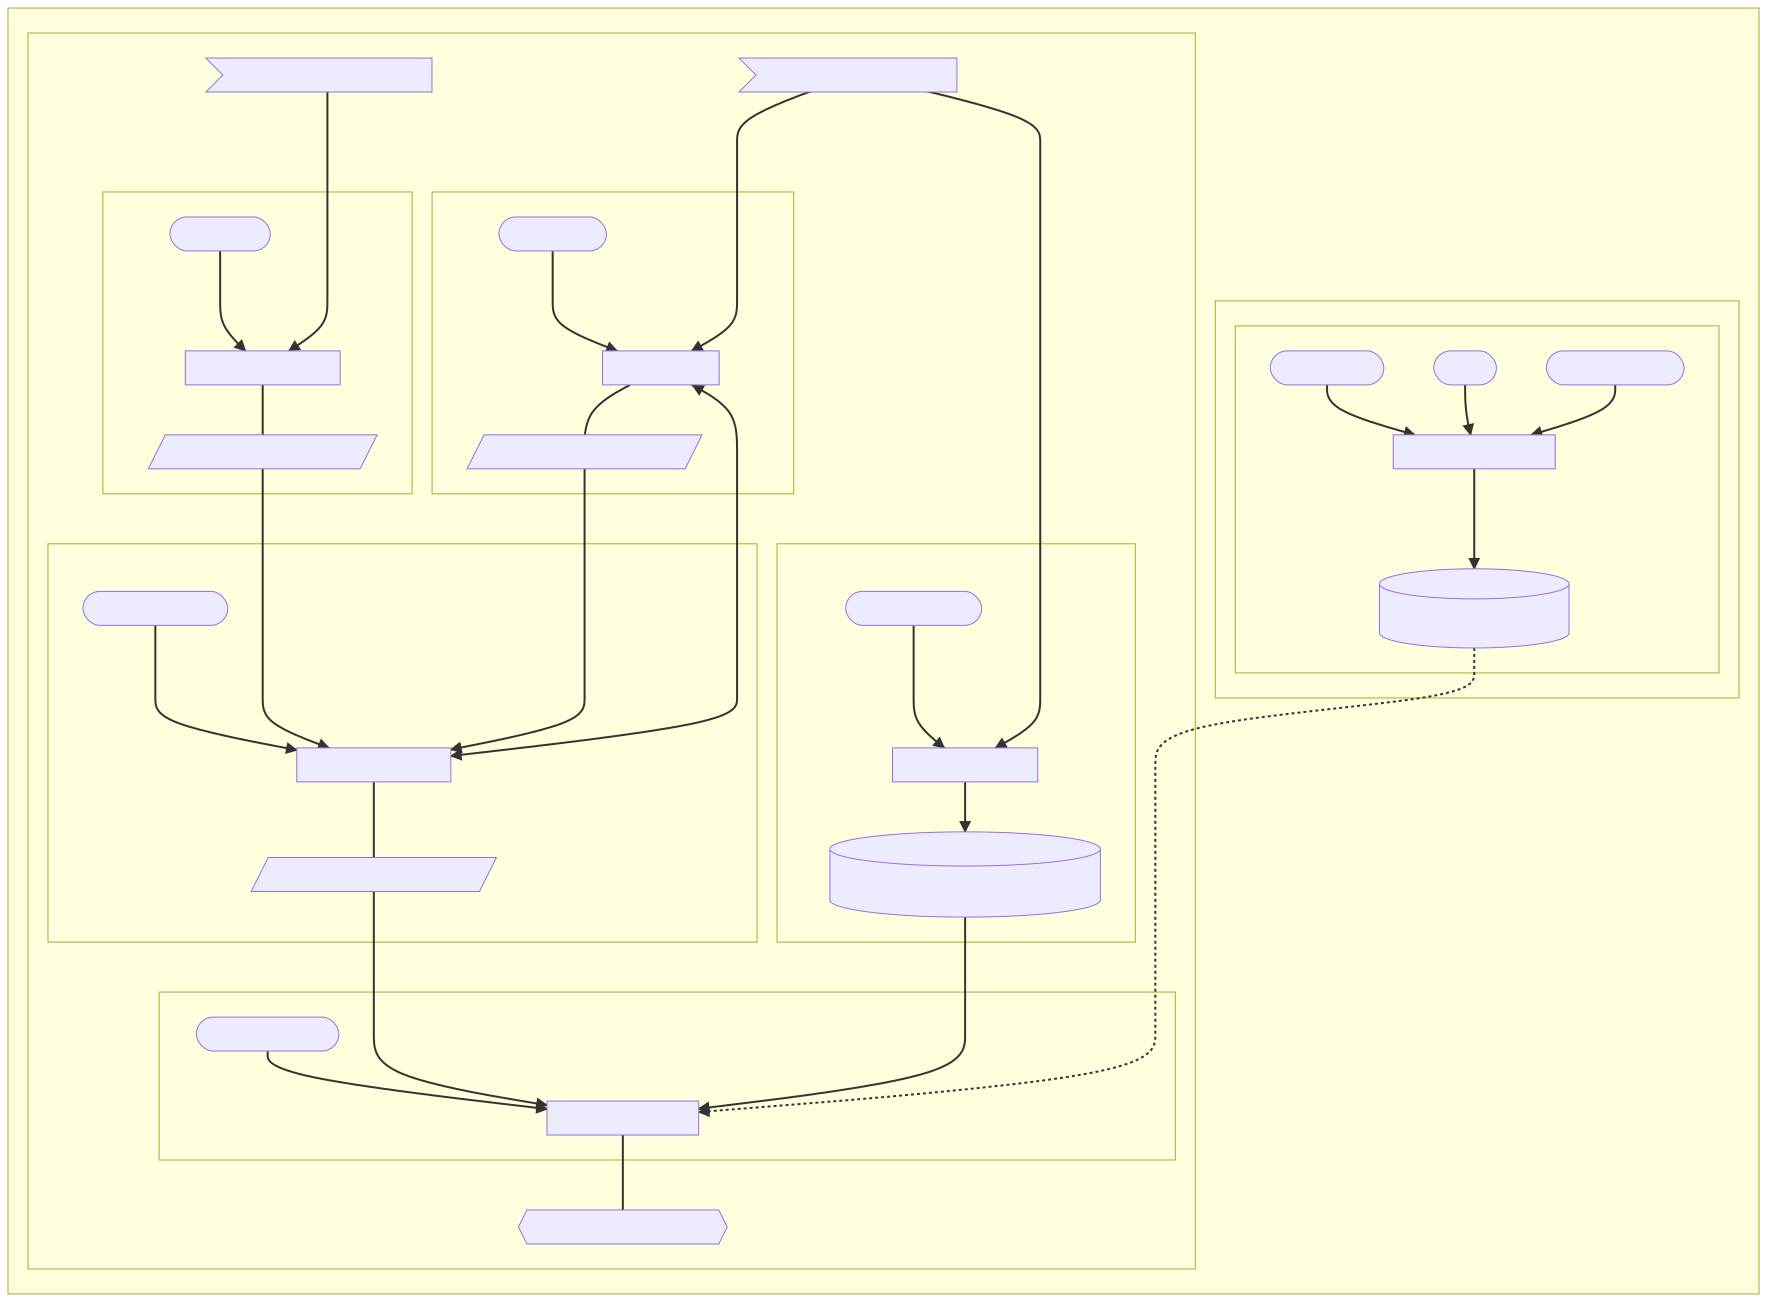
\includegraphics[width=\textwidth]{img/overview.pdf}
    \caption{High-level overview of the design proposal for our application framework}
\end{figure}

\texttt{rt-app}'s design is based around some components which are regarded as standard in the mobile robotics field, such as:
\begin{itemize}
    \item The \textit{pose}, which is the basic unit of data containing all of the information about the orientation and speed of the mobile platform, plus timestamping.
    \item The \textit{odometry}, which constantly elaborates the data received from various sources, such as the mobile platform's wheel encoders, to keep track of where the robot is going.
    \item The \textit{costmap}, which is responsible for determining how likely the robot is to collide with an obstacle, using a predefined map and integrating data from other sources.
    \item The \textit{local planner}, which drives the robot towards a goal using the data provided by the odometry and various other sources, such as AMCL.
    \item \textit{AMCL}, which is a collection of algorithms that use data coming from the sensors, such as a LiDAR, to greatly improve the quality of the localization \cite{roswiki-amcl}.
    \item The \textit{global planner}, which builds a global plan and the costmap from raw data before the real time processes are started.
\end{itemize}

Moreover, the following components have been envisioned:
\begin{itemize}
  \item The \textit{pose manager}, which is a pivotal component that manages the lifecycle of a pose, its duty is to control the flow of data between the modules and to make sure that timestamping is consistent.
  \item The \textit{dispatcher}, which takes care of initializing threads and resources, and is responsible for terminating the application once all workers have finished their job.
\end{itemize}

Most of these operations are to be performed on-line, that is in a real-time fashion, except for global planning and thread dispatching, both of which happen once, when the dispatcher sets the modules up.

\subsection{Kernel}

An integral part of our design revolves around exploiting the capabilities of a real-time operating system: in the Linux world, this can be accomplished through co-kernel solutions, like Xenomai or RTAI, or via the \texttt{PREEMPT\_RT} patch.

The \texttt{PREEMPT\_RT} patch was introduced in 2005 with the goal of reducing the latency and increasing the determinism of the Linux kernel. Since its introduction, the patch has slowly gained traction amongst the kernel developers' community and it's hopefully going to be merged into mainline soon \cite{lwn-rt-future}. Given that the co-kernel approach requires an application to use custom APIs, we've chosen to patch our kernel: this ensures that any program written and compiled on off-the-shelf Linux distributions will run unmodified on a patched kernel, and benefit from it.

The goal of the patch is not making the system faster, but rather to eliminate virtually all of the mechanisms that introduce unbounded latencies in kernel space. By doing this, the RT kernel is able to improve the consistency of the system calls significantly \cite{dmoceri-benchmarking-rtlinux}, albeit with a small performance hit. A formal model of the Linux kernel latencies, and a tool to analyze them have been developed by \textcite{demistifying-rt-latency}.

Nowadays, the impact of \texttt{PREEMPT\_RT} may not be immediately obvious, as many of its features have trickled down from the patch to the mainline kernels over the last 16 years. The most notable examples, from an academic standpoint, are:

\begin{itemize}
    \item The \textit{priority inheritance} system, which attempts to solve the well-discussed problem of priority inversion.
    \item The introduction of \textit{threaded interrupt handlers}, which are necessary to reduce unbounded latencies associated with non-deterministic peripherals such as HIDs.
    %\item The 
\end{itemize}

However, some of the improvements and most configuration options brought on by the patch haven't been merged with mainline yet: this is why the kernel must be patched, reconfigured, and rebuilt from source to fully appreciate its benefits. While this operation is not difficult, it can become very time-consuming, as a full kernel build on commodity hardware may take several hours.

A through analysis of the topics we've briefly covered over this section has been performed by \textcite{survey-preempt-rt}, and it's been instrumental in aligning our expectations with the actual capabilities of a \texttt{PREEMPT\_RT} patched kernel.

\subsection{Scheduler}

The other fundamental part of a real-time system is the scheduler: since kernel 2.6.22, when CFS replaced the older O(1) scheduler as the default scheduler \cite{lwn-cfs-merge}, Linux offers a complex and modular scheduling system based on several independent priority classes. 

\begin{figure}[H]
    \centering
    \includegraphics[width=\textwidth]{img/sched-class.pdf}
    \caption{The relationship between the scheduling classes provided by the Linux kernel}
\end{figure}

In each priority class, there may be a number of different \textit{scheduling policies} that a programmer or a system administrator might choose for a specific workload. In brief: 

\begin{itemize}
    \item \texttt{STOP}: This is the highest priority class, and it's used in kernel space to pin portions of code on specific cores in an SMP setting.
    \item \texttt{DEADLINE}: This class is mostly used to schedule periodic tasks with an EDF algorithm, which is well suited to real-time workloads, such as video decoding and real-time process control.
    \item \texttt{RT}: This is a POSIX standard compatible scheduling class that is used for some latency-sensitive tasks.
    \item \texttt{CFS}: This is the class that's commonly used for all the processes in userspace, and it's the one that uses the \texttt{nice}ness mechanism.
    \item \texttt{IDLE}: This class is responsible for keeping a CPU idling when there are no schedulable tasks left in any queue.
\end{itemize}

For a more detailed description of the scheduling classes, refer to \texttt{sched(7)} \cite{man-sched-7}.

\subsubsection{The \texttt{SCHED\_DEADLINE} scheduling policy}

%% brief history of sched-edf and who's behind it
\texttt{DEADLINE} is a scheduler developed by Dario Faggioli et al. \cite{lwn-faggioli-mail} that's been available in Linux since kernel 3.14 \cite{kn-linux-314}. This scheduler allows the programmer to define and schedule tasks using an Earliest Deadline First (EDF) algorithm, combined with a mechanism called Constant Bandwidth Server (CBS) to perform resource reservation \cite{cbs-algorithm}.

From a programming standpoint, \texttt{SCHED\_DEADLINE} exposes a rich interface to the scheduler that can be used to finely tune the behavior and constraints of a real-time task. The most fundamental parameters that we can tune are: 

\begin{itemize}
    \item The \textit{period}, or the interval at which the scheduler will allow the task to run again after it yielded.
    \item The \textit{deadline}, or the time after which the task has taken too long to complete and the application must take action.
    \item The \textit{runtime}, or the task's expected worst case execution time.
\end{itemize}

The EDF algorithm is well known in academia for its reliability and ability to fully utilize the system's computational resources: as such, this scheduling class is ideal for real-time periodic tasks.\todo{che schifo sto paragrafo madonna}

\section{Implementation}

Due to the nature and time constraints of this project, implementing the whole application would have been impossible: thus, we've decided to focus on a specific subset of functionalities that are fundamental for a robot to be able to move and avoid obstacles. 

More emphasis was put on the fundamental research needed to steer the project in the right direction, and on the real time (threading, timing and scheduling) portions of the framework than on the actual payload: as such, the accuracy of the navigation algorithms is not exactly top-notch, but this was expected.

\subsection{Components}

From a software engineering standpoint, three distinct kinds of components have been devised:
\begin{itemize}
    \item Modules: comprised of both a header and a source file, the modules contain the schedulable units of the application. Each module contains at least an entry point function, which will be executed when scheduling, and a number of other functions necessary to perform one or more specific tasks.   
    \item Helpers: headers that provide inline functions that wrap around system calls and kernel facilities in a standard way.
    \item Adapters: portions of code that provide an high-level interface to an hardware platform like Otto.
\end{itemize}

The only exceptions to this rule are the \texttt{main.c} file, which provides a scheduling facility, and the \texttt{config.h} file, which contains preprocessor definitions used to change the behavior of the application for debugging purposes.

\subsection{Threads and scheduling}

Each module contains a schedulable unit, a portion of code that is capable of running in a separate thread, and a number of scheduling parameters that will be passed to a \texttt{sched\_setattr()} call to modify the scheduling attributes of the module's thread.

This architecture is flexible because it lets the programmer decide how a specific module will be scheduled by the system, and using which scheduler. When using \texttt{SCHED\_DEADLINE}, for example, the programmer can provide a \textit{deadline}, a \textit{runtime} and a \textit{period}: those parameters will be used to control when the thread will be selected for execution and after which amount of time it's expected to terminate (at worst) by the scheduler.

To change the scheduling parameters of a task, the programmer must define a \texttt{sched\_attr} structure containing some information such as what policy to use, how to react to certain events, and data specific to each policy such as a deadline.  

\begin{listing}[H]
\inputminted[frame=single,framesep=10pt]{c}{snippets/sched-attr.c}
\caption{Example of the \texttt{sched\_attr} structure for a task with a deadline of 11ms, and a period of 20ms.}
\end{listing}

The \texttt{SCHED\_FLAG\_DL\_OVERRUN} tells the scheduler that we want a \texttt{SIGXCPU} signal to be generated when a deadline is missed: this is useful because we can define a recovery behavior and extend or override the default handler.

\begin{listing}[H]
\inputminted[frame=single,framesep=10pt]{c}{snippets/dl-miss-handler.c}
\caption{Example of a deadline miss handler.}
\end{listing}

Lastly, the thread must perform a \texttt{sched\_setattr()} call to tell the scheduler that we want to use different scheduling parameters than the default ones: if the user running the program has the appropriate rights, and no errors occur, the call will be successful and the task be migrated by the kernel to \texttt{DEADLINE}'s ready queue for execution.

\begin{listing}[H]
\inputminted[frame=single,framesep=10pt]{c}{snippets/entry-point.c}
\caption{Example of a periodic task scheduled with \texttt{SCHED\_DEADLINE}.}
\end{listing}

%https://lwn.net/Articles/743946/

\subsection{Timing}

As usual with systems interacting with hardware sensors, timing is a critical part of our demonstration: a simple timing system, wrapping the \texttt{clock\_*()} family of system calls, has been implemented to readily provide information such as global time deltas in nanoseconds that can be used to consistently timestamp information coming from the adapters. This collection of inline functions and globals is an helper, and resides into the \texttt{h\_time.h} header. 

To keep track of the time, the Intel x86\_64 (AMD64) architecture provides access to a series of hardware clocks via the \texttt{RDTSC} and \texttt{RDTSCP} instructions. These instructions allow the kernel to query the \texttt{TSC} (Time Stamp Counter) internal register to provide us with a reliable hardware time source. However, the \texttt{TSC} register was introduced with the Pentium architecture and with the advent of technologies like out-of-order execution, hybernation, and multi-core processing it is not advisable to rely on it anymore. This problem, and a number of possible solutions, have been discussed both in official documentation \cite{intel-rdtsc-bench} and articles from notable sources \cite{ms-rdtsc-issues}.

Conveniently, the Linux kernel works around this problem for us: to accurately advance its internal timers the kernel uses several clock sources and an unit of measurement called \textit{jiffy}, which is tied to the value of `HZ` and is fine-tuned to each architecture's needs \cite{elinux-hrts}. Thanks to this complex architecture, which is described in depth by the manual pages \cite{man-clock-getres-2}, we can trust the values provided by system calls such as \texttt{clock\_gettime()} because they're consistent enough to provide us usable values in the tens of nanoseconds range.

Besides keeping a time base and calculating deltas, the \texttt{h\_time} helper mostly performs conversions: since the standard library uses \texttt{timespec} structures to pass values around, \texttt{h\_time} is also responsible for translating \texttt{timespec}s to nanoseconds where needed.  

\subsubsection{Performance and average latency}

To measure the performance of our timing system, a small test suite has been developed. \todo{describe rt-test-suite}

\subsection{Logging}

The problem of logging arose while trying to debug a problem we had with the USAD mobile platform earlier this year: the system experienced a crash, and we were not able to pinpoint a cause because the navigation stack did not use the logging facilities provided by the operating system, but rather was relying on its own approach. This meant that it would've been difficult to precisely determine when a specific error happened in the time domain of the whole system, and in our case that those application logs were completely lost because of a system crash.

To solve this problem, we've decided to use \texttt{syslog()}, which is the standard way to implement logging in Linux: syslog is well documented, performant and its output can be readily analyzed through tools like journalctl.

\subsection{Communications}

As we stated earlier, the \textit{adapters} provide a clean way to interact with various peripherals.

\subsubsection{Serial}

Currently, the demo application issues command to the Otto mobile platform via and FTDI UART using serial communications at 9600 Baud. The \texttt{a\_otto} adapter provides functions that wrap around the read() and write() system calls to communicate with Otto's microcontroller over the serial line: before being sent, the data is encoded using the NanoPB library,  

\subsection{Shared memory}

Not implemented.\todo{remove or what?}

\section{Future Development}

\begin{itemize}
    \item More modules
    \item Better separation of tasks
    \item Code deduplication
\end{itemize}

\newpage
% Ch3
\chapter{Implementation Issues}

During the development of our demo, we've encountered a number of issues that, while not integral to the purpose of this document, have had a notable impact on the design and implementation process of the application: keeping those out of this report wouldn't have been fair, so we've decided to include them in this appendix. 

\section{Patching and building the kernel}

Due to the fact that the preempt-rt patch has still not been mainlined, it was necessary to rebuild the kernel. 

http://kernel-notes.gbittencourt.net/compiling-preempt-rt/

\begin{itemize}
    \item Download https://git.kernel.org/pub/scm/linux/kernel/git/rt/linux-stable-rt.git/tag/?h=v5.4.74-rt41-rebase and untar (~900MB of sources) and cd
    \item \texttt{cp /boot/config-\$(uname -r) .config}
    \item \texttt{make olddefconfig}
    \item \texttt{make -j \$(nproc) deb-pkg}
    \item Wait ~4Hrs
    \item Install the deb pkgs and reboot
\end{itemize}

\section{Emulating the mobile platform}

Due to logistics issues caused by the COVID-19 pandemic, the IRAlab team has not been able to deploy the Otto mobile platform for several months: this posed a serious problem, since we could not use it for developing the \texttt{a\_otto} adapter.

To work around this problem, we've set out to simulate Otto's communication stack by using an ESP8266 (NodeMCU "amica" 1.0) and providing dummy data to the demo's odometry module for testing. 

This eventually caused a deluge of problems, since the two platforms behave in slightly different ways and it was a serious setback.

\section{External impact on RT performance}

\subsection{Processor features and hardware components}
\begin{itemize}
    \item Caches
    \item CPU Threads (SMT)
    \item CPU Cores (SMP)
    \item Intel Management Engine (ME) and AMD Secure Platform (PSP)
    \item Power saving states, suspension, hybernation and clock boost
\end{itemize}

CPUSETS solve the problem of SMP (and SMT, to some extent) by locking specific processes (as in thread groups) to a partition of the available processors (or cores).

\subsection{Filesystem and I/O performance}

% Tail
\printbibliography
\end{document}